\newpage

\section{Семинар 1}

\subsection{Пример неизмеримого множества}

Возьмем окружность $S$, $r_S = 1$, $\mu(S) = 2\pi$

Возьмем $\alpha$ такое, что $\frac{\alpha}{\pi}$ --- иррационально.

Рассмотрим $R_{n\alpha},\ n \in \Z$.

Орбита точки $x$ $O(x) = \left\{ R_{nx}(x) : n \in \Z\right\}$

$x \sim y$, если $y = R_{nx}(x)$ для некоторого $n$. Или же $O(x) = O(y)$

Возьмем по одному представителю из каждого класса эквивалентности. Тогда полученное множество $E_0$ неизмеримо.

$$E_n = R_{n\alpha}(E_0),\ n \in \Z$$

\begin{itemize}
  \item $\bigcup_{\Z} E_n = S$
  \item $E_n \cap E_m = \emptyset\ (n \ne m)$
  \item $\mu(E_n) = \mu(E_0)$
\end{itemize}

$$2\pi = \mu(S) = \mu\left(\bigcup_{\Z} E_n\right) = \sum_{\Z} \mu(E_0)$$

Последнее, в зависимости от $\mu(E_0)$ либо 0, либо $\infty$.

Получаем противоречие.


\subsection{Канторово множество $C$}

Из единичного отрезка 
$C_{0}=[0,\ 1]$ удалим среднюю треть, то есть интервал 
$(\frac{1}{3},\ \frac{2}{3})$. Оставшееся точечное множество обозначим через 
$C_{1}$. Множество $C_{1}=[0,\ \frac{1}{3}] \cup [\frac{2}{3},\ 1]$ состоит из двух
отрезков; удалим теперь из каждого отрезка его среднюю треть, и оставшееся множество обозначим через 
$C_{2}$. Повторив эту процедуру опять, удаляя средние трети у всех четырёх отрезков, получаем 
$C_{3}$. Дальше таким же образом получаем последовательность замкнутых множеств
$\displaystyle C_{0}\supset C_{1}\supset C_{2}\supset \dots $. Пересечение
$C=\bigcap _{i=0}^{\infty }C_{i}$
называется канторовым множеством.

Свойства:
\begin{itemize}
  \item Канторово множество имеет меру $\mu = 0$ (доказывается подсчетом суммы длин удаляемых интервалов)
  \item $C$ замкнуто
  \item $C$ нигде не плотно
  \item $C$ имеет мощность континуума
\end{itemize}

Докажем последнее утверждение. Для этого воспользуемся троичной записью числа.
Тогда числа из $C$ записываются в троичной записи только цифрами $0$ и $2$. Но таких чисел столько же, сколько существует двоичных записей
чисел на $[0, 1]$. Получается $C \equiv [0, 1]$



\subsection{Неравенства Юнга, Гёльдера и Минковского}

$p, q > 1 : \frac{1}{p} + \frac{1}{q} = 1$

\begin{wrapfigure}{r}{0.4\textwidth}
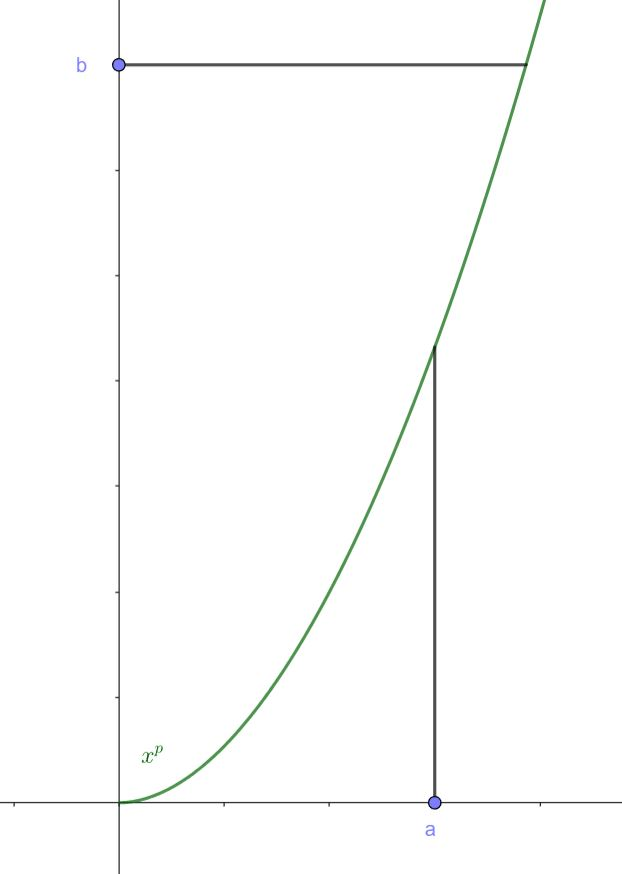
\includegraphics[width = 0.4\textwidth]{images/ung.JPG}
\end{wrapfigure}

\begin{theorem}[Юнг]
  $ab \leq S_1 + S_2 = \int_{0}^{a} x^{p-1} dx + \int_0^b x^{q-1} dx = \frac{a^p}{p} + \frac{b^q}{q}$
\end{theorem}

\begin{theorem}[Гёльдер]
  $a = (a_1, a_2, \dots, a_n)$

  $b = (b_1, \dots, b_n)$

  $$\sum_{i = 1}^{n} |a_ib_i| \leq \left(\sum_{i=1}^n |a_i|^p \right)^{\frac{1}{p}} \cdot \left(\sum_{i=1}^n |b_i|^q \right)^{\frac{1}{q}}$$
\end{theorem}

\begin{proof}
  В силу однородности имеем право предположить, что $\sum_{i=1}^n |a_i|^p =$\\$= \sum_{i=1}^n |b_i|^q = 1$.

  По неравенству Юнга
  
  $$\sum_{i = 1}^{n} |a_ib_i| \leq \sum_{i = 1}^n \left( \frac{a_i|^p}{p} + \frac{|b_i|^q}{q}\right) =
  \frac{1}{p}\sum |a_i|^p + \frac{1}{q} \sum |b_i|^q = 1$$
\end{proof}

\textbf{Замечание 1.} При $n \to \infty$ получим неравенство для рядов.

\textbf{Замечание 2.} Имеется аналог неравенства Гёльдера для интегралов

\begin{theorem}
  $$\int_X |fg|\ d\mu \leq \left(\int_X |f|^p\ d\mu \right)^\frac{1}{p} \cdot \left(\int_X |g|^q\ d\mu \right)^\frac{1}{q}$$
\end{theorem}